\section{Results}
\label{results}
Both the BVH builder and path tracer were implemented in Go and only utilize the CPU. Code is optimized moderately without exploiting any SIMD instructions. A series of tests was conducted to compare the build times, ray tracing performance and resulting time per frame rendered between different hyperparameter configurations. LBVH was used as reference, PHR-Fast and PHR-HQ used the parameters proposed by Hendrich et al.\cite{hendrich_parallel_2017}, namely $\alpha=0.5, \delta=6$ and $\alpha=0.55, \delta=9$, respectively. PHR-Grid uses parameters based on the proposed grid search approach over the search space $\alpha\in\{0.4,0.45,0.5.0.55\}, \delta\in\{6,7,8,9\}$ and PHR-BO uses parameters resulting from a Bayesian optimization over the equivalent interval $\alpha\in[0.4,0.55], \delta\in[6,9]$. The Bayesian optimization itself is executed utilizing the bo framework\cite{ou19bo} and is based on a Gaussian process and expected improvement as exploration strategy. 

To make results more reliable, all numbers were averaged over ten executions using the bench framework\cite{ou20bench}. Furthermore, the CPU, an AMD Ryzen 2600 eight core processor with 3.4 GHz, was locked to 90 percent capacity to prevent irregularities due to overheating or other high performance fluctuations. Note that the deviation percentages are left out for clarity in the tables presented in this thesis, but the full results are available in the attached files. 

Render times are also averaged over three representative views for each scene. To keep times in an interactive window, only the relatively small resolutions 256x256 and 512x512 were tested with one sample per pixel. 
\subsection{Multi-Bounding Volume Hierarchies}
\label{multi_bvh}
As mentioned in section \ref{phr_algorithm}, the PHR algorithm allows the construction of bounding volume hierarchies with higher branching factors, which is especially useful for SIMD path tracers. Even though the evaluated path tracer does not utilize any SIMD instructions, I compared the build and trace performance of different multi-BVHs. As expected, the performance difference between branching factors was insignificant in most cases. 4-ary BVHs had slightly faster trace times, while 16-ary BVH construction was slightly slower. The following tests were all performed on 2-ary BVHs. 
\subsection{Frame Performance}
The main part of the experiment was about comparing the resulting frame times of all configurations. Table \ref{tab:frametime} shows build time, SAH cost, average render time over the compared view points and the resulting frame times. Note that the PHR build times do not include construction of the auxiliary bounding volume hierarchy, as those would be reused over several frames. 

First of all, the numbers clearly show the impact different PHR parameters can have on the build and trace time of the algorithm. PHR-Fast was indeed fairly fast, but the achieved trace speed is even below the baseline, LBVH, in some cases. PHR-HQ had the fastest trace speed in most cases, but the high build duration often leads to higher frame times. A noticeable difference can be seen between the different scene types. PHR performed comparably worse in single object scenes like Bunny, Dragon and Happy Buddha, often not exceeding the render performance of LBVH by much. Sibenik's and Sponza's render times on the other hand, were improved more significantly by applying PHR. Finally, PHR-Grid and PHR-BO were able to improve frame times significantly in a number of cases. However, Bayesian optimization delivered rather inconsistent results and no approach was able to find the optimal parameters in every case. This is probably a result of overfitting the evaluation function and their parameters to certain scenes. Nonetheless, both PHR-Grid and PHR-BO are able to improve frame times compared to PHR-Fast and PHR-HQ. Figure \ref{fig:difference} shows the average relative performance compared to LBVH in percent. While PHR-Fast only improves frame times by 33\% on average, both optimization approaches surpass an average improvement of 50\%.
\begin{figure} [H]
    \centering
    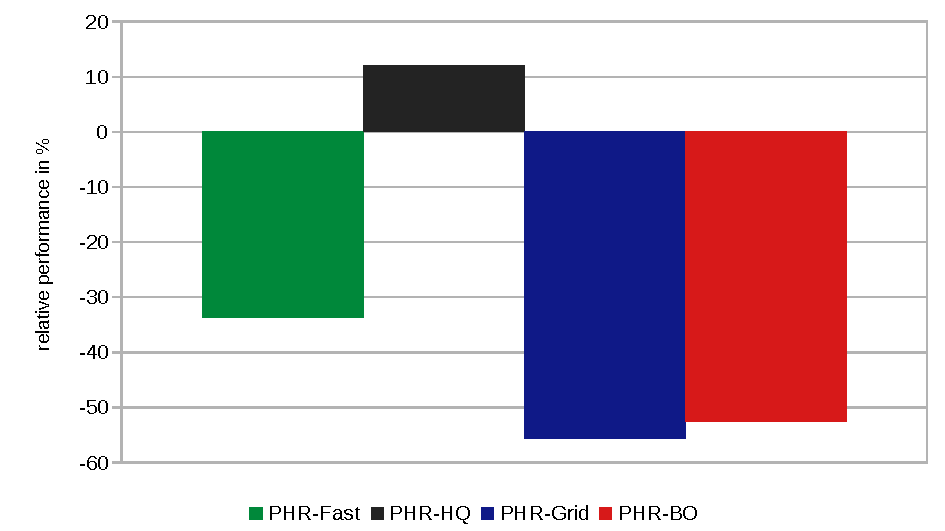
\includegraphics[width=300pt]{images/performance_difference.pdf}
    \caption{Relative difference to LBVH in percent.}
    \label{fig:difference}
\end{figure}
\subsection{Optimization Performance}
Figure \ref{fig:optimization} shows optimization times divided through average frame time, or in other words, how many frames could potentially be rendered instead of executing the optimization. Considering that the average performance increase of both methods amounted around 50\%, i.e. can potentially half the rendering time, optimizations start to become viable at half a frames duration and below. So even though the search space used in grid search is relatively low, the achieved times never reached what would be feasible in interactive applications. Bayesian optimization performed considerably better, but only reached competitive times in a few cases. Note that reaching this time does not equal a performance increase but just a hypothetical chance that frame times are increased. 

This shows that the presented optimization approaches still lack in performance and are not yet viable. PHR needs to be executed to evaluate the cost function, which is especially costly for parameters that result in high build times. This could be improved by limiting the search spacer further or making it dynamic and related to the scene's complexity. An interrupt after a maximum execution time might also be a solution. Bayesian optimization uses a costly run with maxed out parameters to determine the maximum build cost. This could be solved by reusing max values from previous optimizations. This topic is discussed further in section \ref{discussion_execute}.
\begin{figure}[H]
    \centering
    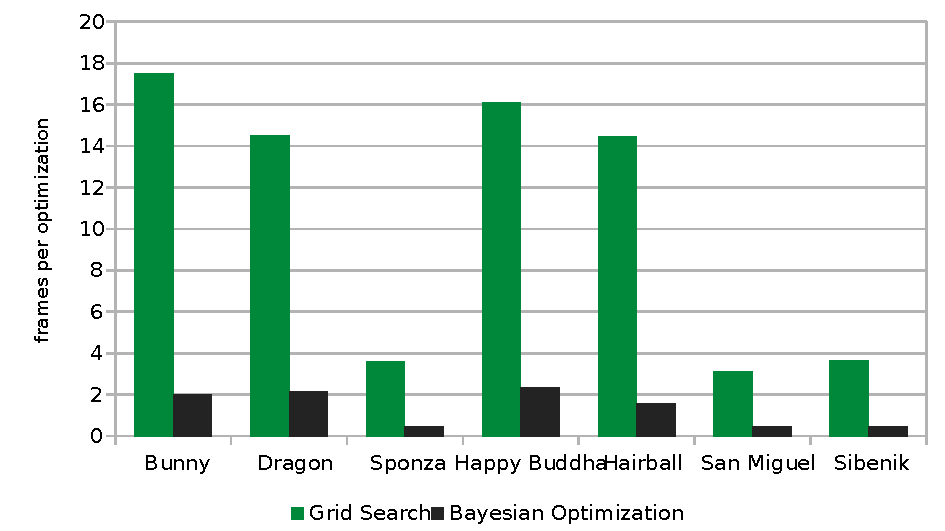
\includegraphics[width=300pt]{images/frame_per_optimization.pdf}
    \caption{Number of potential frames during optimization.}
    \label{fig:optimization}
\end{figure}
\clearpage
\begin{table}
\caption{Performance comparison of a representative selection of tested configuration at 256x256 resolution.}
\label{tab:frametime}
\centering
\begin{tabular}{ | c | m{3.5em} | m{3.5em} | m{3.5em} | m{3.5em} | m{3.5em} |  m{3.5em}|}
\hline
& build time (ms) & render time (ms) & frame time ms & build time (ms) & render time (ms) & frame time ms\\
\hline
& \multicolumn{1}{|m{4.5em}}{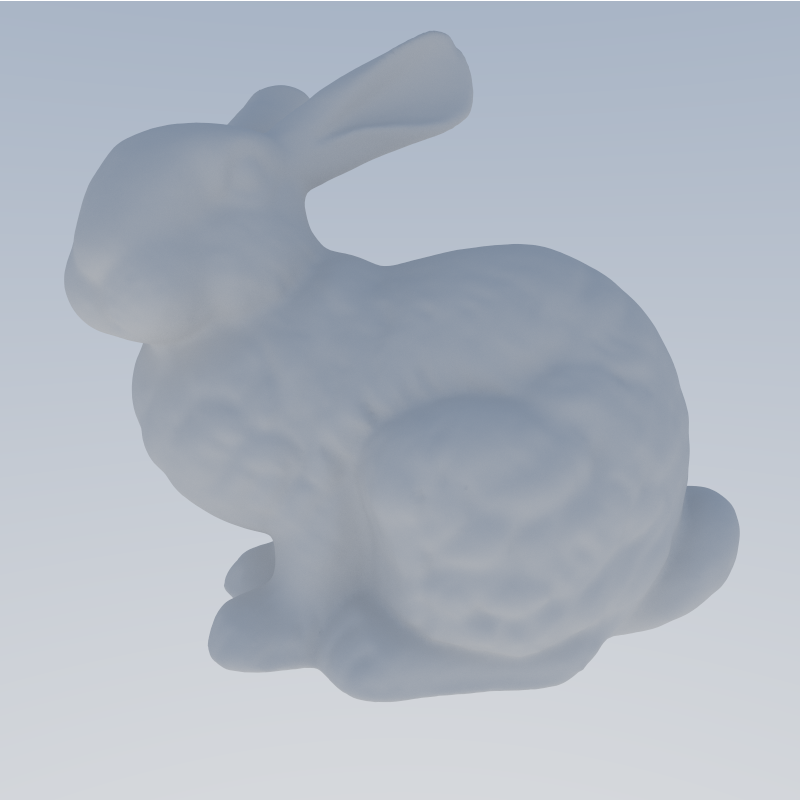
\includegraphics[width=60pt]{images/bunny.png}} &     \multicolumn{2}{m{4em}|}{Bunny \#triangles 144k} 
& \multicolumn{1}{|m{4.5em}}{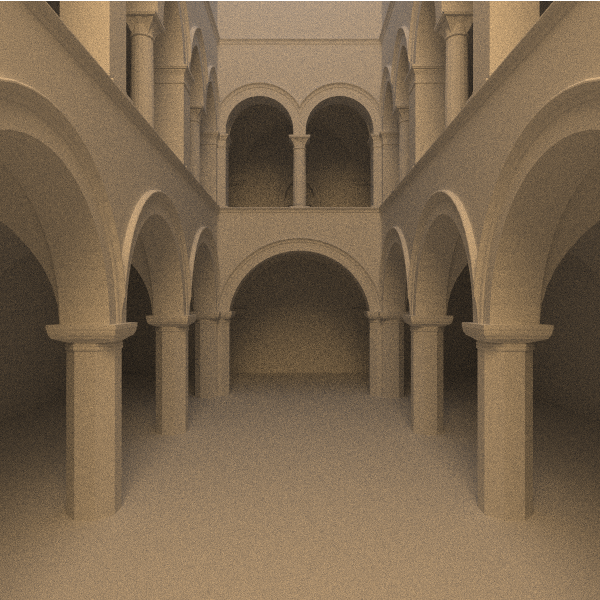
\includegraphics[width=60pt]{images/sponza.png}} & \multicolumn{2}{m{4em}|}{Sponza \#triangles 66k}\\
\hline
LBVH & 152.0 & 21.9 & 173.9            & 70.4 & 227.0 & 297.5 \\
PHR-Fast & 70.5 & 20.1 & 90.6          & 27.6 & 184 & 211.6 \\
PHR-HQ & 273.0 & 20.7 & 293.7          &  94.7 & 182 & 276.7\\
\hline
PHR-Grid & 14.4 & 20.8 & 35.2        &  17.2 & 207 & 224.2\\
PHR-BO & 14.2 & 20.7 & 34.97         &  21.7 & 200 & 221.7\\
\hline
& \multicolumn{1}{|m{4.5em}}{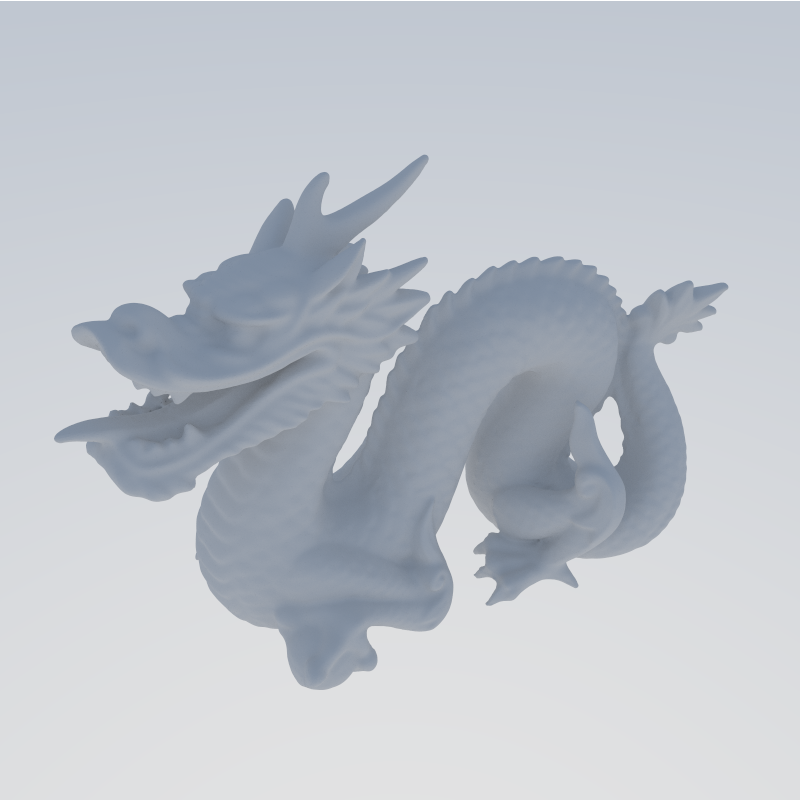
\includegraphics[width=60pt]{images/dragon.png}} &     \multicolumn{2}{m{4em}|}{Dragon \#triangles 817k}

& \multicolumn{1}{|m{4.5em}}{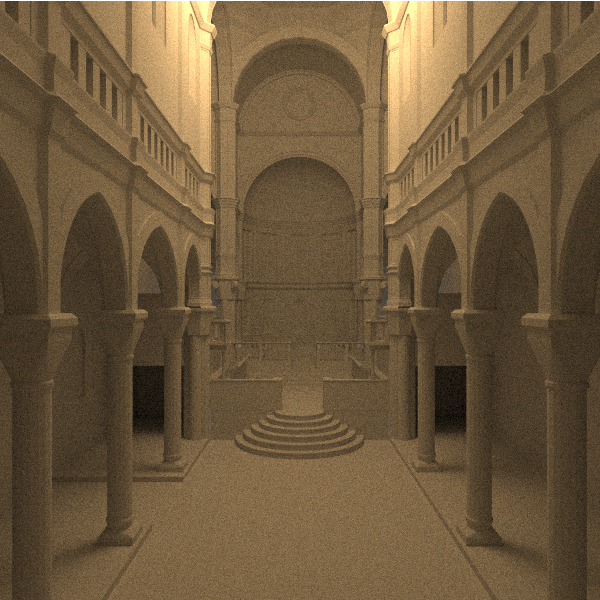
\includegraphics[width=60pt]{images/sibenik.png}} & \multicolumn{2}{m{4em}|}{Sibenik \#triangles 75k}\\

\hline
LBVH & 900.0 & 28.1 & 928.2              &  72.1 & 226.1 & 298.1\\
PHR-Fast & 150.0 & 32.5 & 182.5            &  32.5 & 205 & 237.5\\
PHR-HQ & 1090.0 & 29.0 & 1119.0              &  98.4 & 187  &285.4\\
\hline
PHR-Grid & 31.7 & 63.5 & 95.2            & 19.1 & 236 & 255.1  \\
PHR-BO & 30.8 & 66.1 & 96.9              & 28.1 & 220 & 248.1 \\
\hline
& \multicolumn{1}{|m{4.5em}}{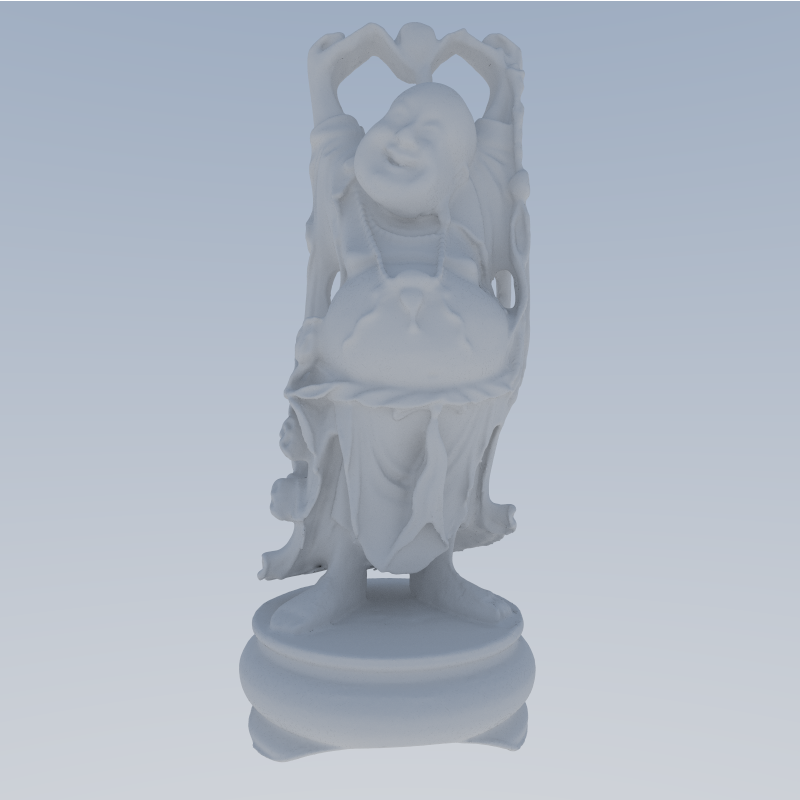
\includegraphics[width=60pt]{images/buddha.png}} & \multicolumn{2}{m{4em}|}{Happy Buddha \#triangles 1087k}

& \multicolumn{1}{|m{4.5em}}{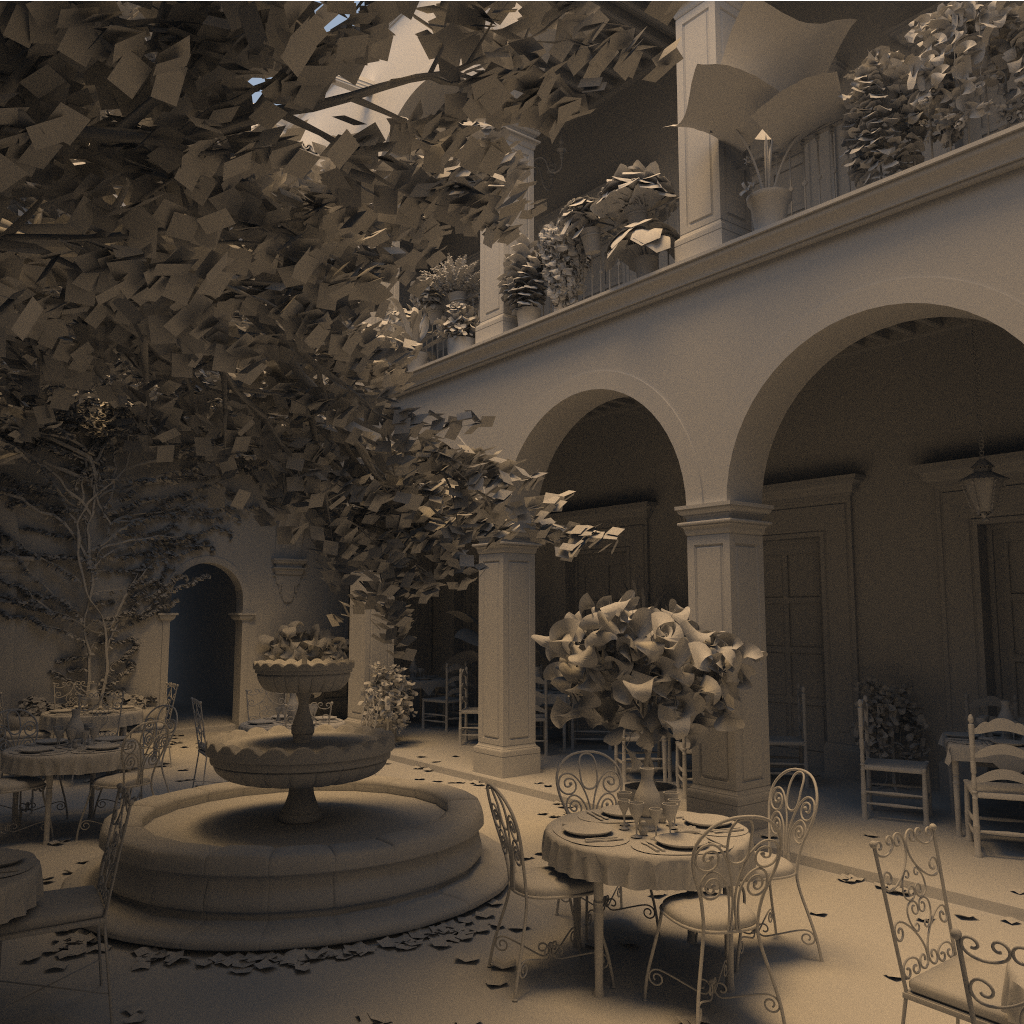
\includegraphics[width=60pt]{images/san_miguel.png}} &     \multicolumn{2}{m{4.5em}|}{San Miguel \#triangles 5617k}\\


\hline
LBVH & 1080 & 25 & 1105                    & 6010.0 & 816.0 & 6826.6 \\                   
PHR-Fast & 190 & 27.6 & 217.6                   & 432.0 & 7830.0 & 8262.0 \\
PHR-HQ & 1250 & 23.7 & 1273.7                     & 2600.0 & 812.3 & 3412.3 \\
\hline
PHR-Grid & 40.5 & 57.5 &98                   & 1300.0 & 1856.6 & 3156.6  \\
PHR-BO & 42.1 &58 &100.1                     & 815.0 & 3203.3 & 4018.3 \\
\hline
\end{tabular}
\end{table}
\cleardoublepage